%%% Template originaly created by Karol Kozioł (mail@karol-koziol.net) and modified for ShareLaTeX use

\documentclass[a4paper,fleqn,11pt]{article}

\usepackage[T1]{fontenc}
\usepackage[utf8]{inputenc}
\usepackage{graphicx}
\usepackage{xcolor}

\usepackage{tgtermes}

\usepackage[
pdftitle={EE698G - Probabilistic Mobile Robotics Assignment}, 
pdfauthor={Satya Prakash Panuganti, 14610},
colorlinks=true,linkcolor=blue,urlcolor=blue,citecolor=blue,bookmarks=true,
bookmarksopenlevel=2]{hyperref}
\usepackage{amsmath,amssymb,amsthm,textcomp}
\usepackage{enumerate}
\usepackage{multicol}
\usepackage{tikz}

\usepackage{geometry}
\geometry{total={210mm,297mm},
left=25mm,right=25mm,%
bindingoffset=0mm, top=20mm,bottom=20mm}

\usepackage{ mathrsfs }
\usepackage{ upgreek }
\linespread{1.3}

\newcommand{\linia}{\rule{\linewidth}{0.5pt}}

% custom theorems if needed
\newtheoremstyle{mytheor}
    {1ex}{1ex}{\normalfont}{0pt}{\scshape}{.}{1ex}
    {{\thmname{#1 }}{\thmnumber{#2}}{\thmnote{ (#3)}}}

\theoremstyle{mytheor}
\newtheorem{defi}{Definition}

% my own titles
\makeatletter
\renewcommand{\maketitle}{
\begin{center}
\vspace{2ex}
{\huge \textsc{\@title}}
\vspace{1ex}
\\
\linia\\
\@author \hfill \@date
\vspace{4ex}
\end{center}
}
\makeatother
%%%

% custom footers and headers
\usepackage{fancyhdr,lastpage}
\pagestyle{fancy}
\lhead{}
\chead{}
\rhead{}
\lfoot{Assignment 4}
\cfoot{}
\rfoot{Page \thepage\ /\ \pageref*{LastPage}}
\renewcommand{\headrulewidth}{0pt}
\renewcommand{\footrulewidth}{0pt}
%

%%%----------%%%----------%%%----------%%%----------%%%

\begin{document}

\title{EE698G - Probabilistic Mobile Robotics Assignment}

\author{Satya Prakash Panuganti, 14610}

\date{26 March, 2017}

\maketitle

\section{EKF \& UKF}

\subsection{EKF}

\subsubsection{Typical run of EKF-localization with default config parameters :}

\begin{center}
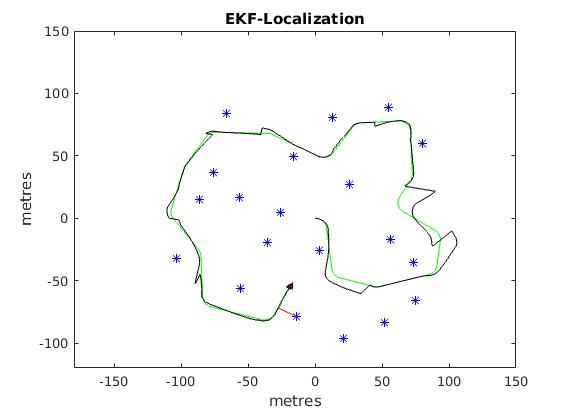
\includegraphics[scale = 0.74]{../images/EKF-default1.jpg} \\
\end{center}

\begin{center}
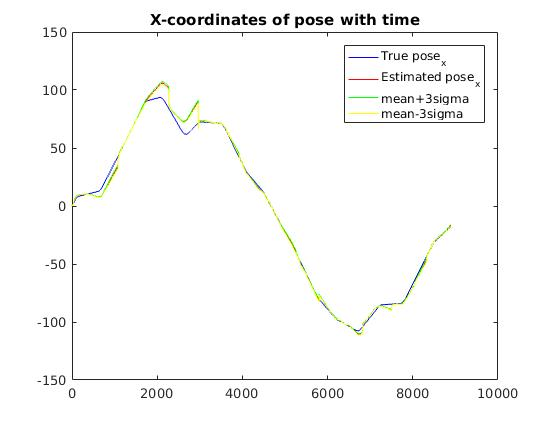
\includegraphics[scale = 0.37]{../images/EKF-default1-xvt.jpg}
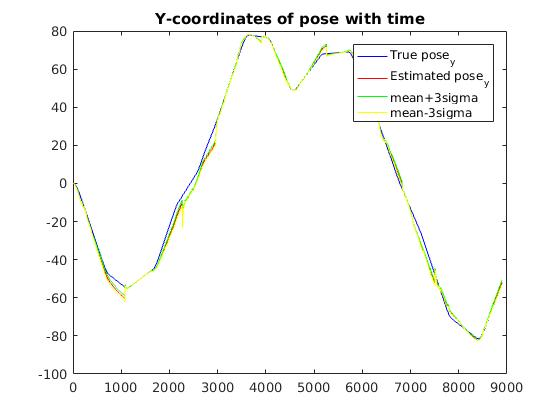
\includegraphics[scale = 0.37]{../images/EKF-default1-yvt.jpg}
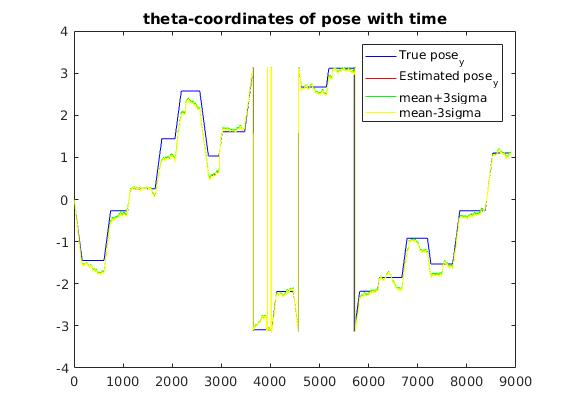
\includegraphics[scale = 0.37]{../images/EKF-default1-avt.jpg}
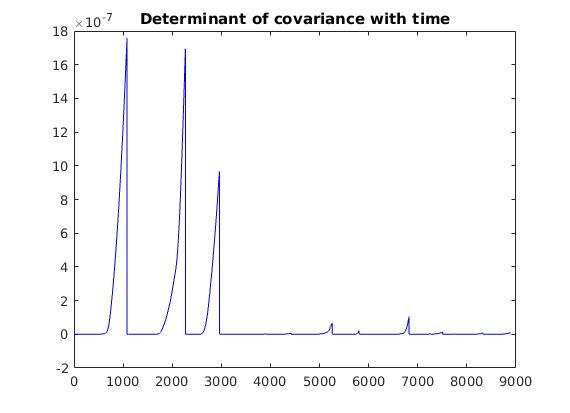
\includegraphics[scale = 0.37]{../images/EKF-default1-cvt.jpg}
\end{center}

\subsubsection{Typical run of EKF-localization with perfect control (No control noise) :}

\begin{center}
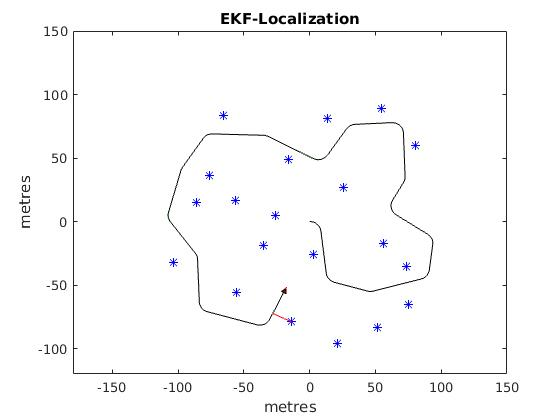
\includegraphics[scale = 0.74]{../images/EKF-perfect-control.jpg} \\
\end{center}

\begin{center}
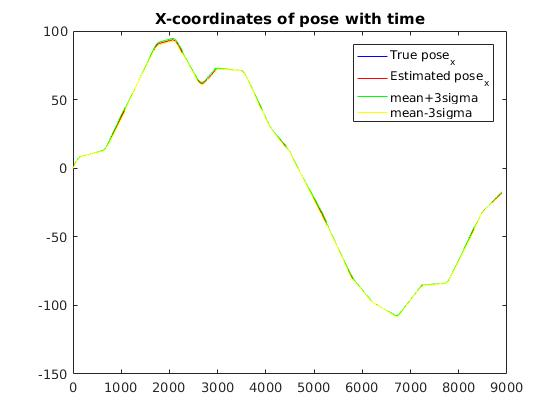
\includegraphics[scale = 0.37]{../images/EKF-perfect-control-xvt.jpg}
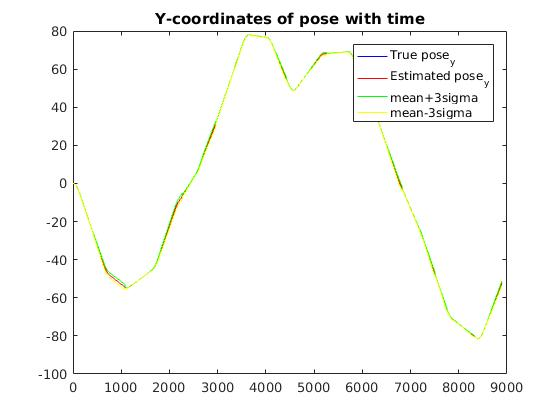
\includegraphics[scale = 0.37]{../images/EKF-perfect-control-yvt.jpg}
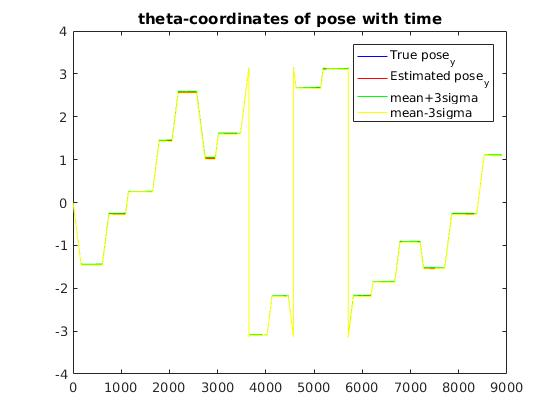
\includegraphics[scale = 0.37]{../images/EKF-perfect-control-avt.jpg}
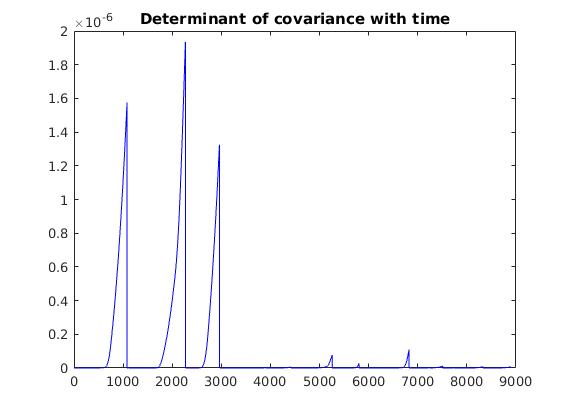
\includegraphics[scale = 0.37]{../images/EKF-perfect-control-cvt.jpg}
\end{center}

\subsubsection{Typical run of EKF-localization with perfect measurements (No measurement noise) :}

\begin{center}
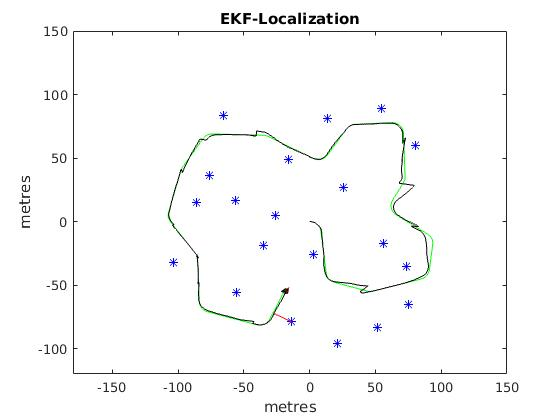
\includegraphics[scale = 0.74]{../images/EKF-perfect-measurement.jpg} \\
\end{center}

\begin{center}
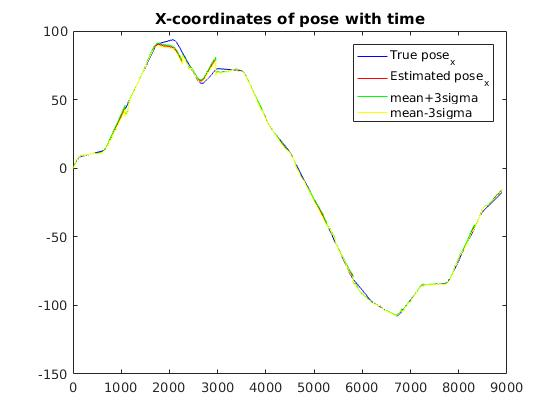
\includegraphics[scale = 0.37]{../images/EKF-perfect-measurement-xvt.jpg}
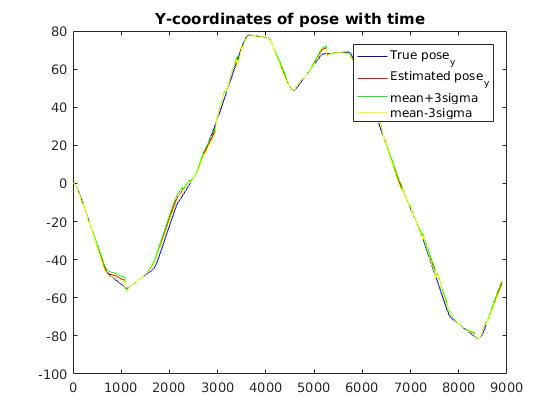
\includegraphics[scale = 0.37]{../images/EKF-perfect-measurement-yvt.jpg}
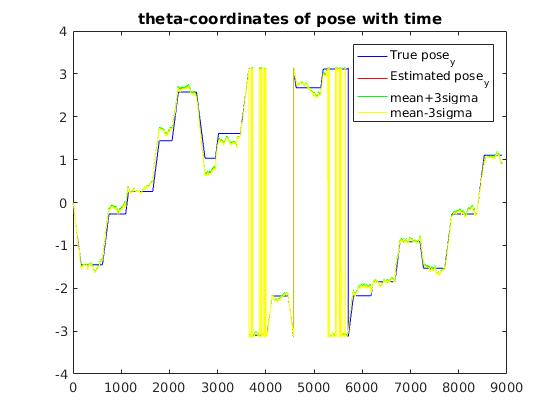
\includegraphics[scale = 0.37]{../images/EKF-perfect-measurement-avt.jpg}
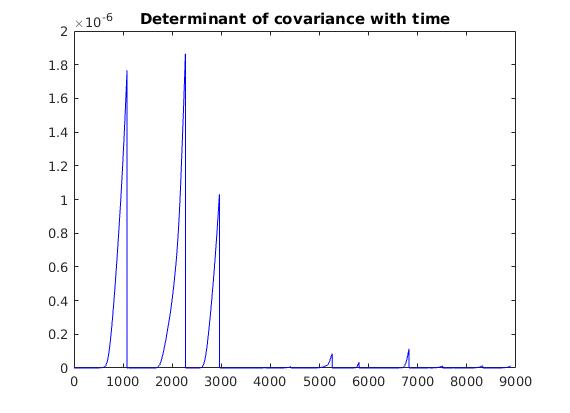
\includegraphics[scale = 0.37]{../images/EKF-perfect-measurement-cvt.jpg}
\end{center}

\subsection{UKF}

All runs were performed with :
\begin{align*}
	\alpha & = 0.001 \\
	\beta  & = 2 \\
	\lambda & = -0.9
\end{align*}

\subsubsection{Typical run of UKF-localization with default config parameters :}

\begin{center}
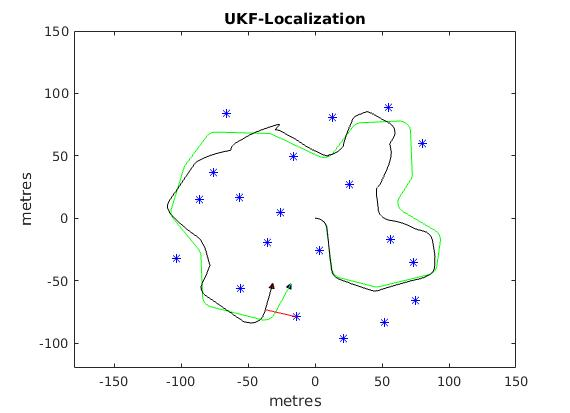
\includegraphics[scale = 0.74]{../images/UKF-default1.jpg} \\
\end{center}

\begin{center}
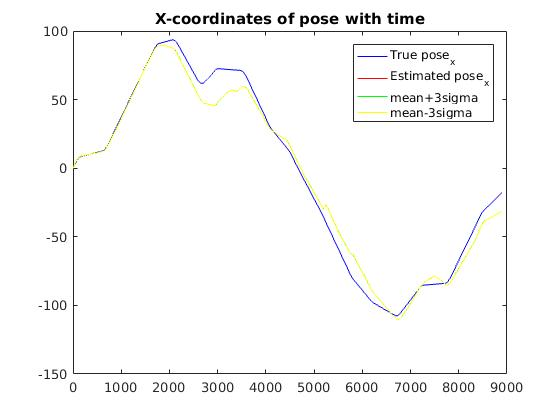
\includegraphics[scale = 0.37]{../images/UKF-default1-xvt.jpg}
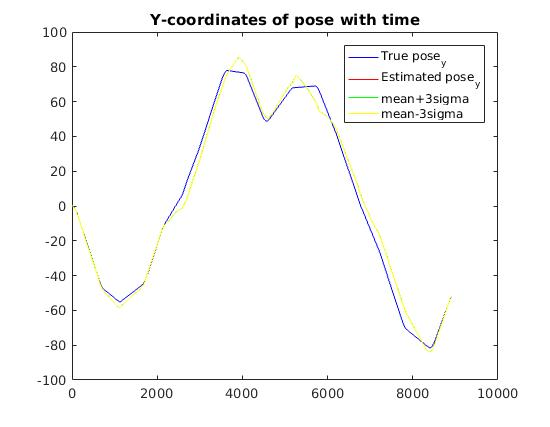
\includegraphics[scale = 0.37]{../images/UKF-default1-yvt.jpg}
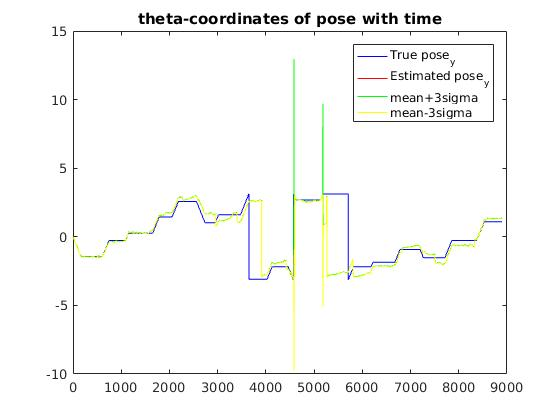
\includegraphics[scale = 0.37]{../images/UKF-default1-avt.jpg}
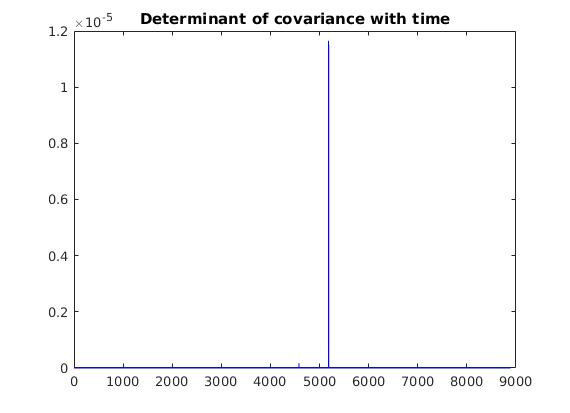
\includegraphics[scale = 0.37]{../images/UKF-default1-cvt.jpg}
\end{center}

\begin{align*}
Error = \begin{bmatrix}
			 819.2356\\
			 485.2469\\
			 159.7805
		\end{bmatrix}
\end{align*}

\subsubsection{Typical run of UKF-localization with perfect control (No control noise) :}

\begin{center}
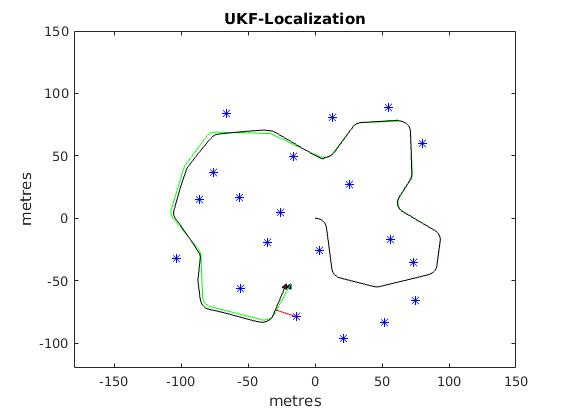
\includegraphics[scale = 0.74]{../images/UKF-perfect-control.jpg} \\
\end{center}

\begin{center}
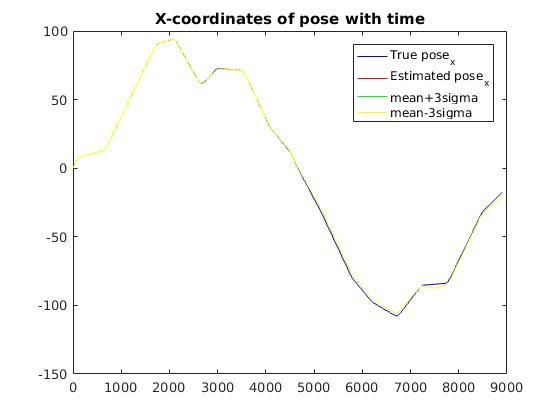
\includegraphics[scale = 0.37]{../images/UKF-perfect-control-xvt.jpg}
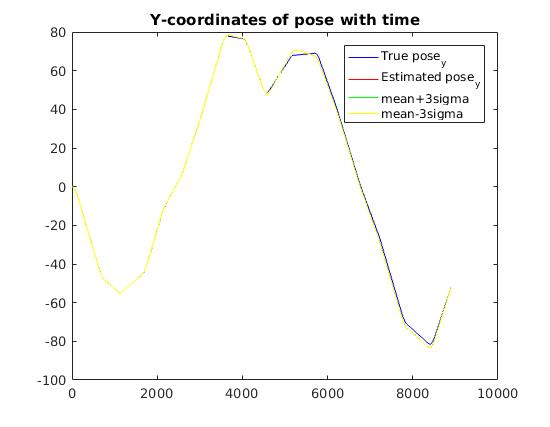
\includegraphics[scale = 0.37]{../images/UKF-perfect-control-yvt.jpg}
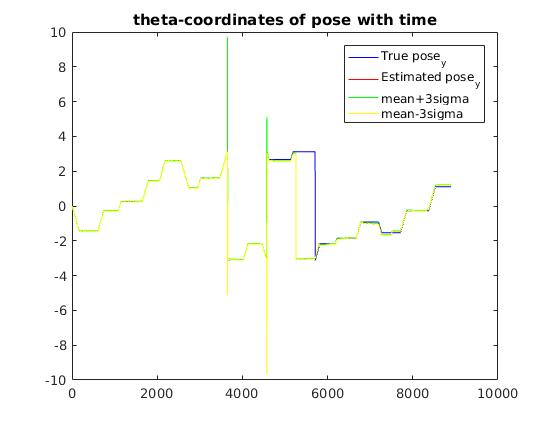
\includegraphics[scale = 0.37]{../images/UKF-perfect-control-avt.jpg}
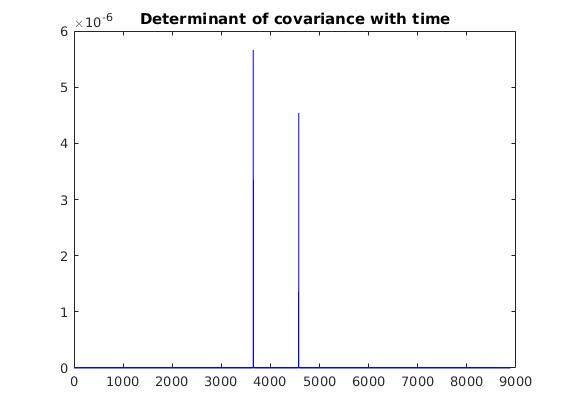
\includegraphics[scale = 0.37]{../images/UKF-perfect-control-cvt.jpg}
\end{center}

\begin{align*}
Error = \begin{bmatrix}
			117.1791\\
			106.9854\\
			131.8872
  		\end{bmatrix}
\end{align*}

\subsubsection{Typical run of UKF-localization with no noise :}

\begin{center}
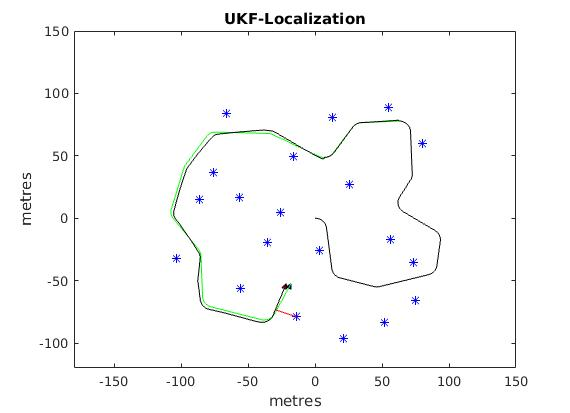
\includegraphics[scale = 0.74]{../images/UKF-no-noise.jpg} \\
\end{center}

\begin{center}
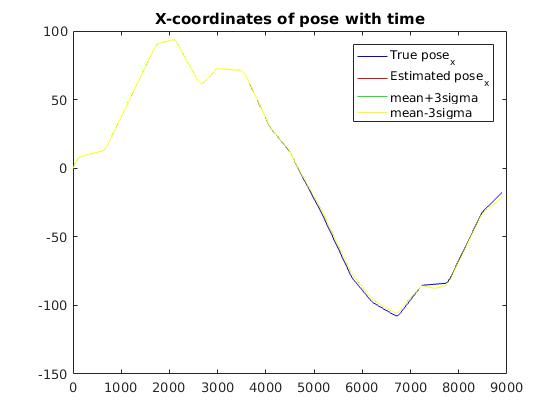
\includegraphics[scale = 0.37]{../images/UKF-no-noise-xvt.jpg}
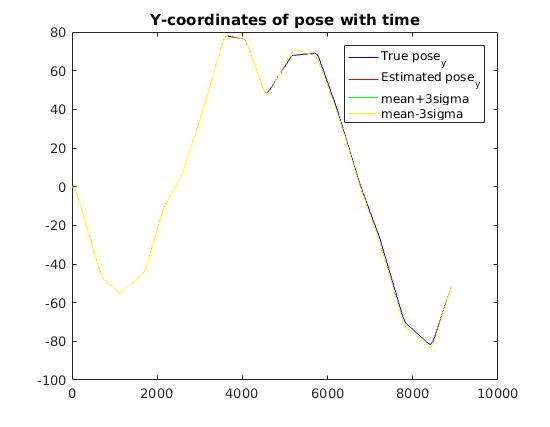
\includegraphics[scale = 0.37]{../images/UKF-no-noise-yvt.jpg}
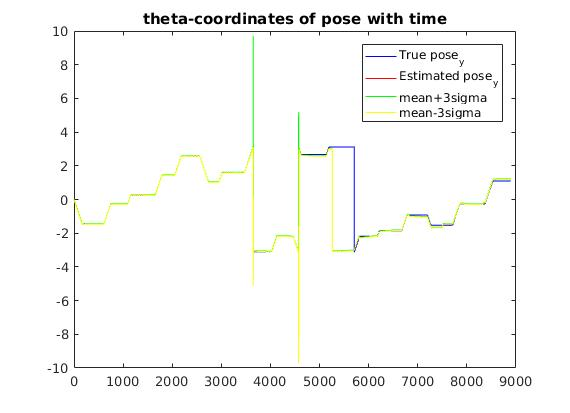
\includegraphics[scale = 0.37]{../images/UKF-no-noise-avt.jpg}
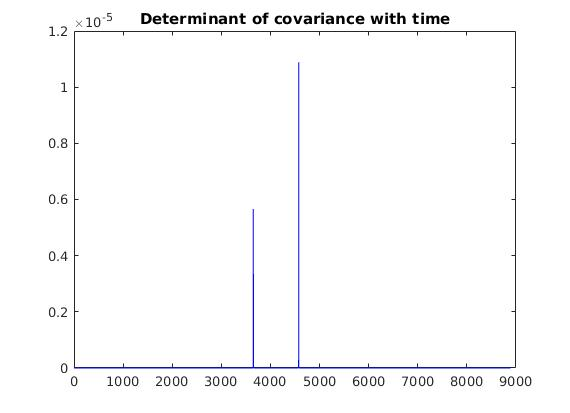
\includegraphics[scale = 0.37]{../images/UKF-no-noise-cvt.jpg}
\end{center}

\begin{align*}
Error = \begin{bmatrix}
			118.6433 \\
			108.3882 \\
			131.9377
		\end{bmatrix}
\end{align*}

\subsection{Comments and Observations on EKF and UKF Localization :}

EKF is simpler to work when it is possible to compute the gradient of the measurement and state functions. Its simplicity lies in the fact that there are no parameters such as $\alpha, \beta, \lambda$ which need to be tuned in EKF. Furthermore, EKF is also easier to implement if one has the Jacobians for the state and measurement models on hand. \\
Hence, in cases where EKF is sufficient for state estimation, I would refrain from using the UKF. I haven't been able to tune my implementation of UKF, but I feel that on chosing proper UKF parameters, it can out perform EKF, especially in situations where computation of the Jacobian is not possible.\\
The highly non-linear state model appears to be posing a problem on the introduction of control noise. Both EKF and UKF seem to fail because they attempt to fit a uni-modal probability distrubution to a non-linear problem.

\pagebreak

\section{Particle Filter}

\subsection{Result with Number of Particles = 1}

\begin{center}
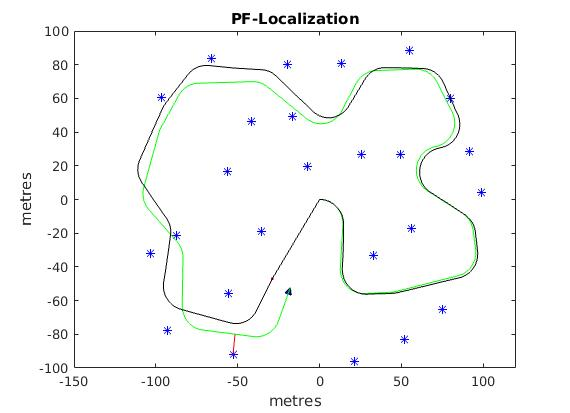
\includegraphics[scale = 0.74]{../images/PF-num1.jpg} \\
\end{center}

\subsection{Result with Number of Particles = 5}

\begin{center}
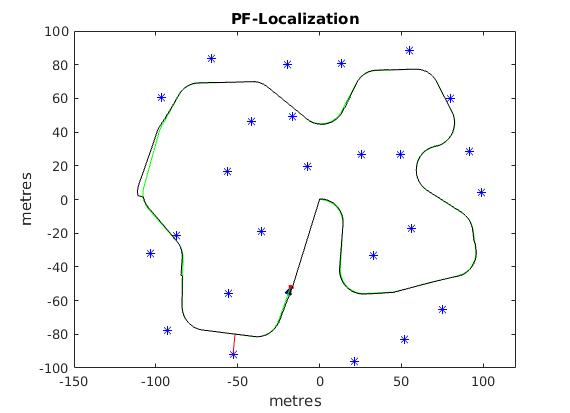
\includegraphics[scale = 0.74]{../images/PF-num5.jpg} \\
\end{center}

\subsection{Result with Number of Particles = 20}

\begin{center}
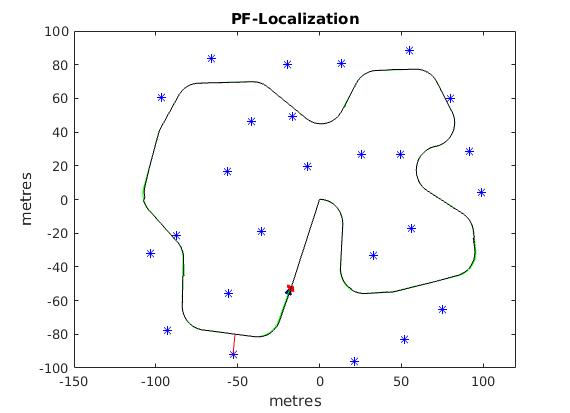
\includegraphics[scale = 0.74]{../images/PF-num20.jpg} \\
\end{center}

\subsection*{Findings}

Particle Filter is simple to implement. From my experiment with the above problem, it appears that it is possible to get good results with a moderate number of particles. It can also be be inferred from the above results that the state estimation tends to improve with an increase in the number of particles. Results obatined from particle filter appear to be better than those from EKF / UKF for highly nonlinear problems since it doen't attempt to fit a unimodal distribution for the state. Another advantage of using particle filter to perform localication is that one can choose the number of particles based on the available computing resources. Hence, it is always possible to improve the quality of state estimation simply by increasing the number of particles provided sufficient resources are available. In methods such as UKF, tuning of parameters, which can become a time consuming process, must be done in order to improve the estimation.

\end{document}